
\documentclass[8pt]{article}

\usepackage[utf8]{inputenc}

\usepackage{amsmath}
\usepackage{graphicx}
\usepackage{amssymb}
\usepackage{float}
% set font size to 11pt


\setlength{\parskip}{\baselineskip}%
\setlength{\parindent}{0pt}%

\begin{document}

\title{Extended Coursework Report}
\author{lwp26}
\date{Feburary 2023}
\maketitle

\begin{abstract}
    \centering
    % Optimisation of tuned dampers to reduce the amplitude of resonant responses of a 3 degree of freedom structure
    In this report a model structure with 3 degrees of freedom will be hamonically excited to determine the resonant frequencies and mode shapes of the structure.
    The resonant frequnencies and mode shapes will be used to determine optimal design parameters for three seperate absorbers to reduce the resonant responses at each mode shape.
    % The optimal design parameters will be determined by using a genetic algorithm to minimise the resonant response of the structure.
    This approach can be used on real structures to reduce the amplitude of their resonant response to earthquakes.
\end{abstract}

\section{Introduction}

% Aims, Objectives and context
% context

Modern structures are designed to withstand a range of distributed static loads however they are vulnerable to harmonic excitations such as earthquakes.


\subsection{Aims}

\begin{itemize}
\item To determine the resonant frequencies of a 3 degree of freedom structure
\item To determine the properties of three seperate tuned mass dampers to reduce the three resonant response of the structure
\item To investigate the combined effect of the tuned mass dampers on the resonant response of the structure
\end{itemize}

\section{Methodology and theory}
% Summary of theory and information to reproduce

The structure experimented on in this report has 3 floors stacked on top of each other connected by springs.
Resonant frequencies were determined by performing a sweep of harmonic excitations on the structure and recording the responses at each frequency.
These undamped responses were then saved and used for comparison with the responses of the structure after the addition of tuned mass dampers.

The tune mass damper model used is a simple spring-mass-damper system with a spring stiffness $k$ and damping coefficient $\lambda$.
The position of the damper is also important as it must be ideally placed at an anti node of the resonant mode shape.
For each mass spring damper the stiffness, $k$, must be tuned to match the resonant frequency of the structure.
\begin{equation}
    k = m\omega_n^2
\end{equation}
The spring used is effectively a cantilever which has a stiffness
\begin{equation}
    k = \frac{W}{\delta} = \frac{3EI}{L^3}
\end{equation}
Equating these gives the length of the cantilever as
\begin{equation}
    L = \sqrt[3]{\frac{3EI}{m\omega_n^2}}
\end{equation}
This did not however give optimal results for a variety of reasons, the main one being that the equation for deflection
of a cantilever assumes small deflections and the deflection of the tuned mass damper is significant.
The method used for tuning was to incrementally change the stiffness of the spring by changing its length until the response 
at the resonant frequency was at a minimum. 

A single mass of 50g was added to the end of the cantilever spring and the structures response was tested with the mass at the top and 1cm below the top.
In the 1st mode the response was worse when the mass was positioned 1cm from the top and so two more 50g masses were added until the resonant response decreased.
This was done such that the optimal length lies on the cantilever for fine tuning. It can also be seen in equation (3) that increasing $m$
decreases the optimal length of the cantilever such that the tuned mass dampers resonant frequency matches that of the building.
The other modes did not require this as a single 50g mass was sufficient to 

The damping coefficient was effectively unchanged as this is caused by the viscous friction of the air on the mass.

\newpage

\section{Results}

\begin{figure}[H]
    
    \centering
    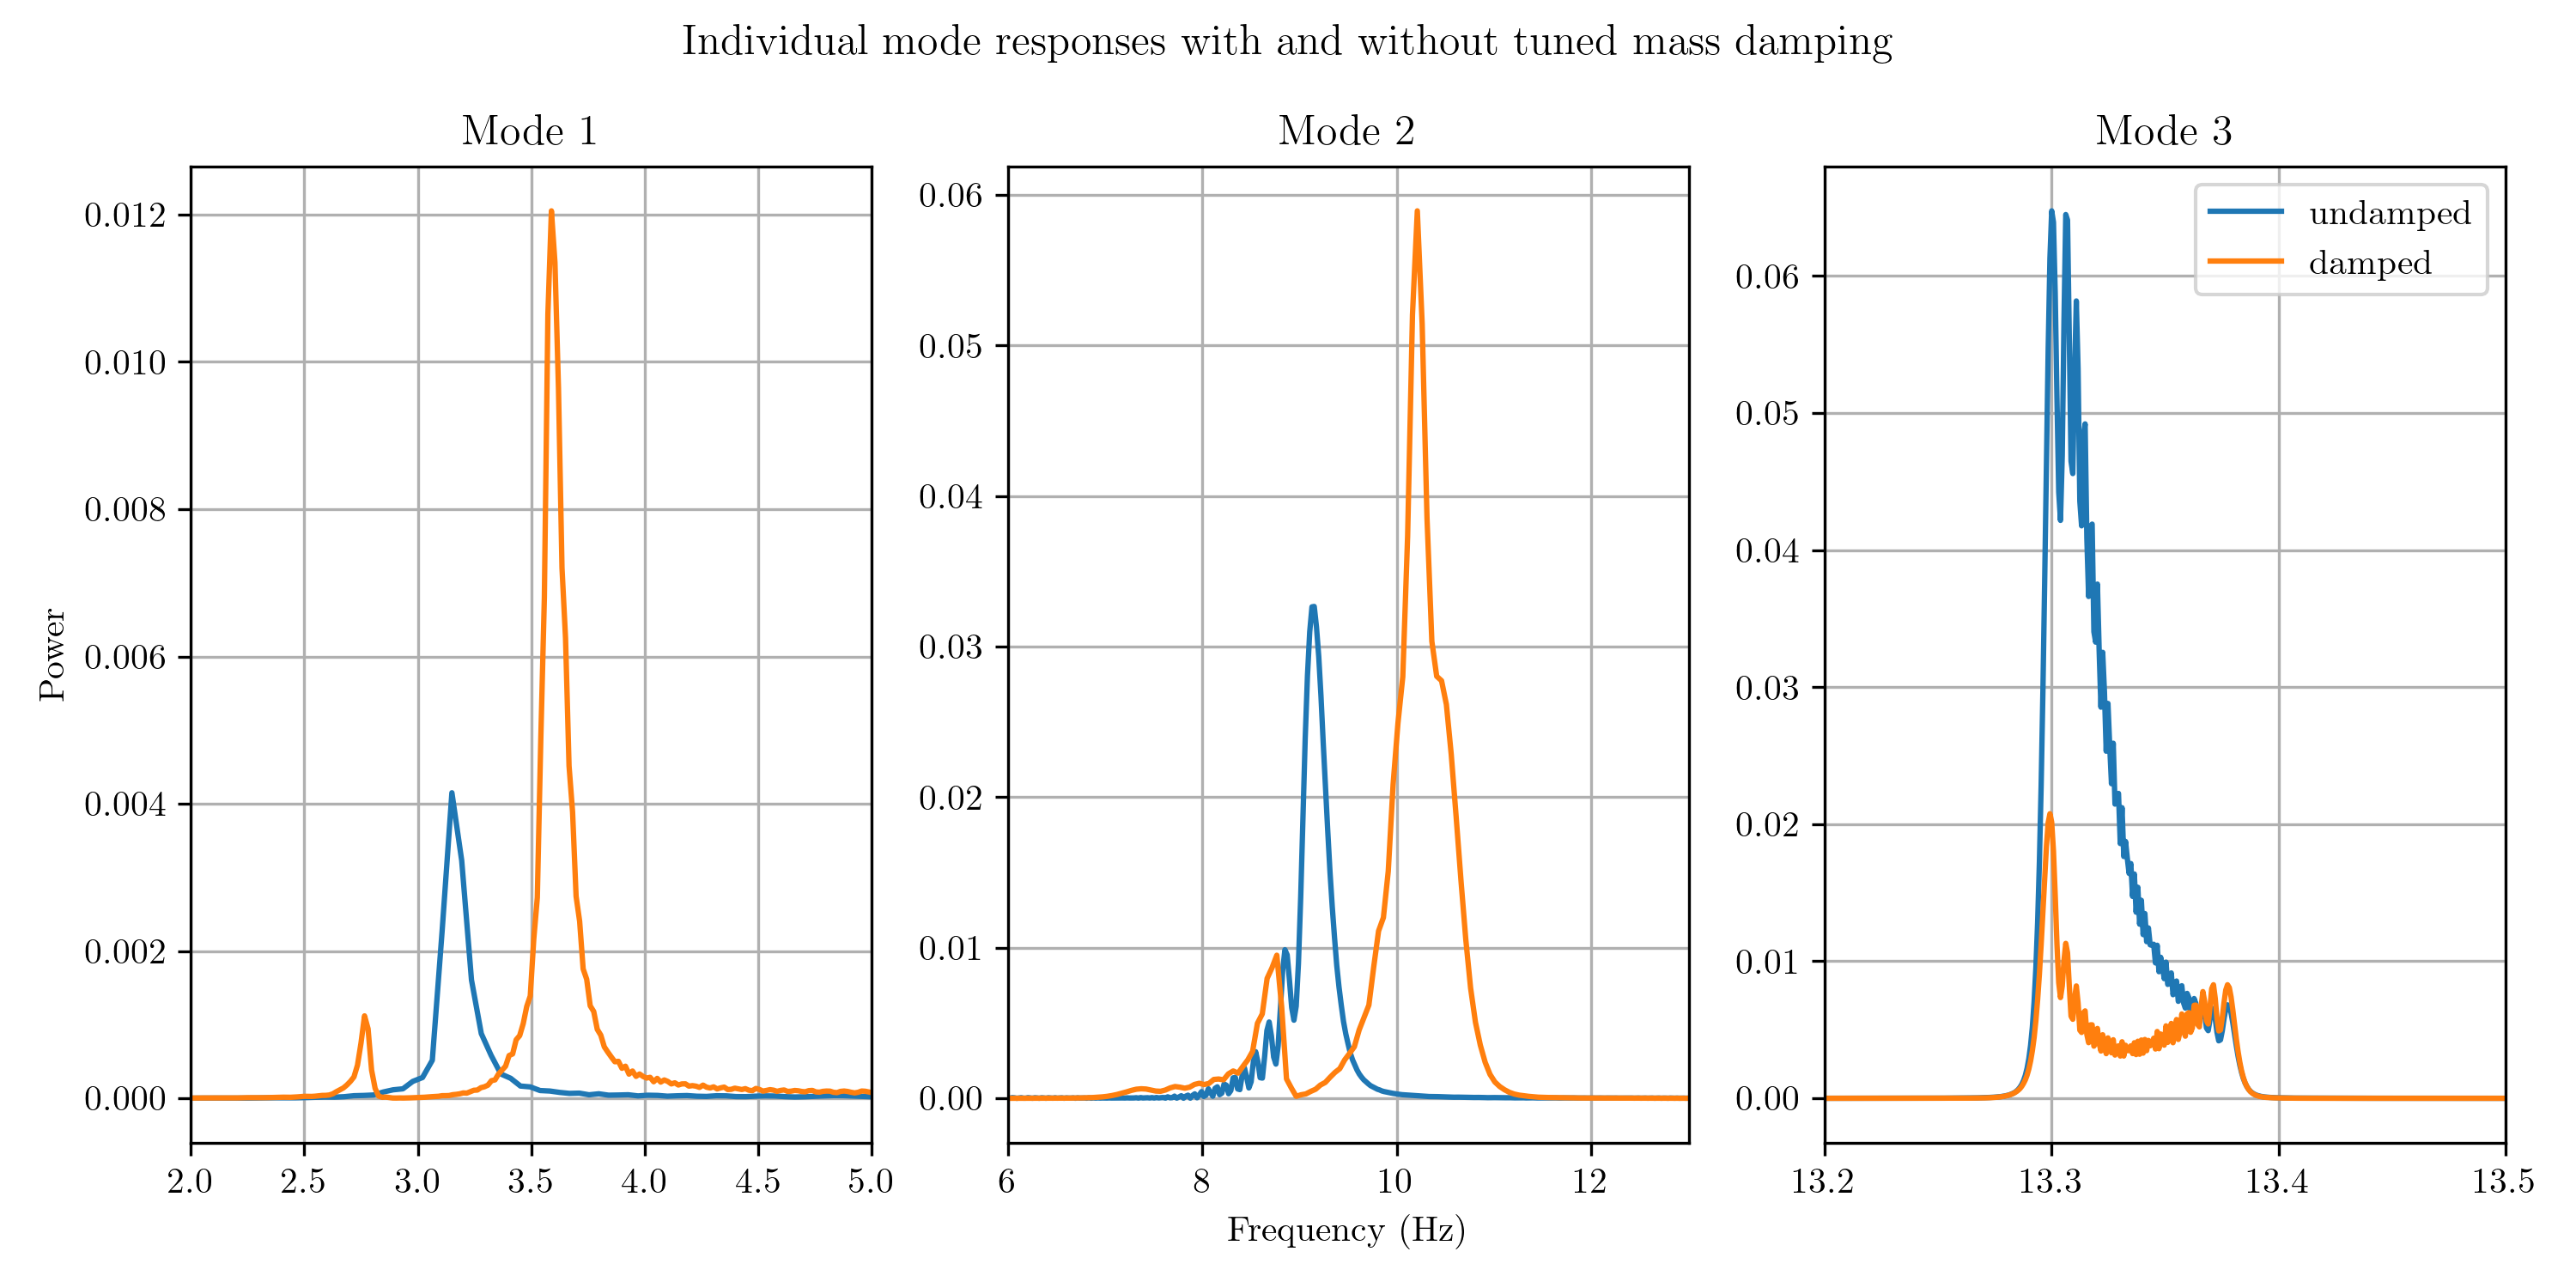
\includegraphics[width=1\textwidth]{modes.png}
    \caption{\label{fig:modes} Harmonic responses of each node before and after the addition of a single tuned damper to that node}
    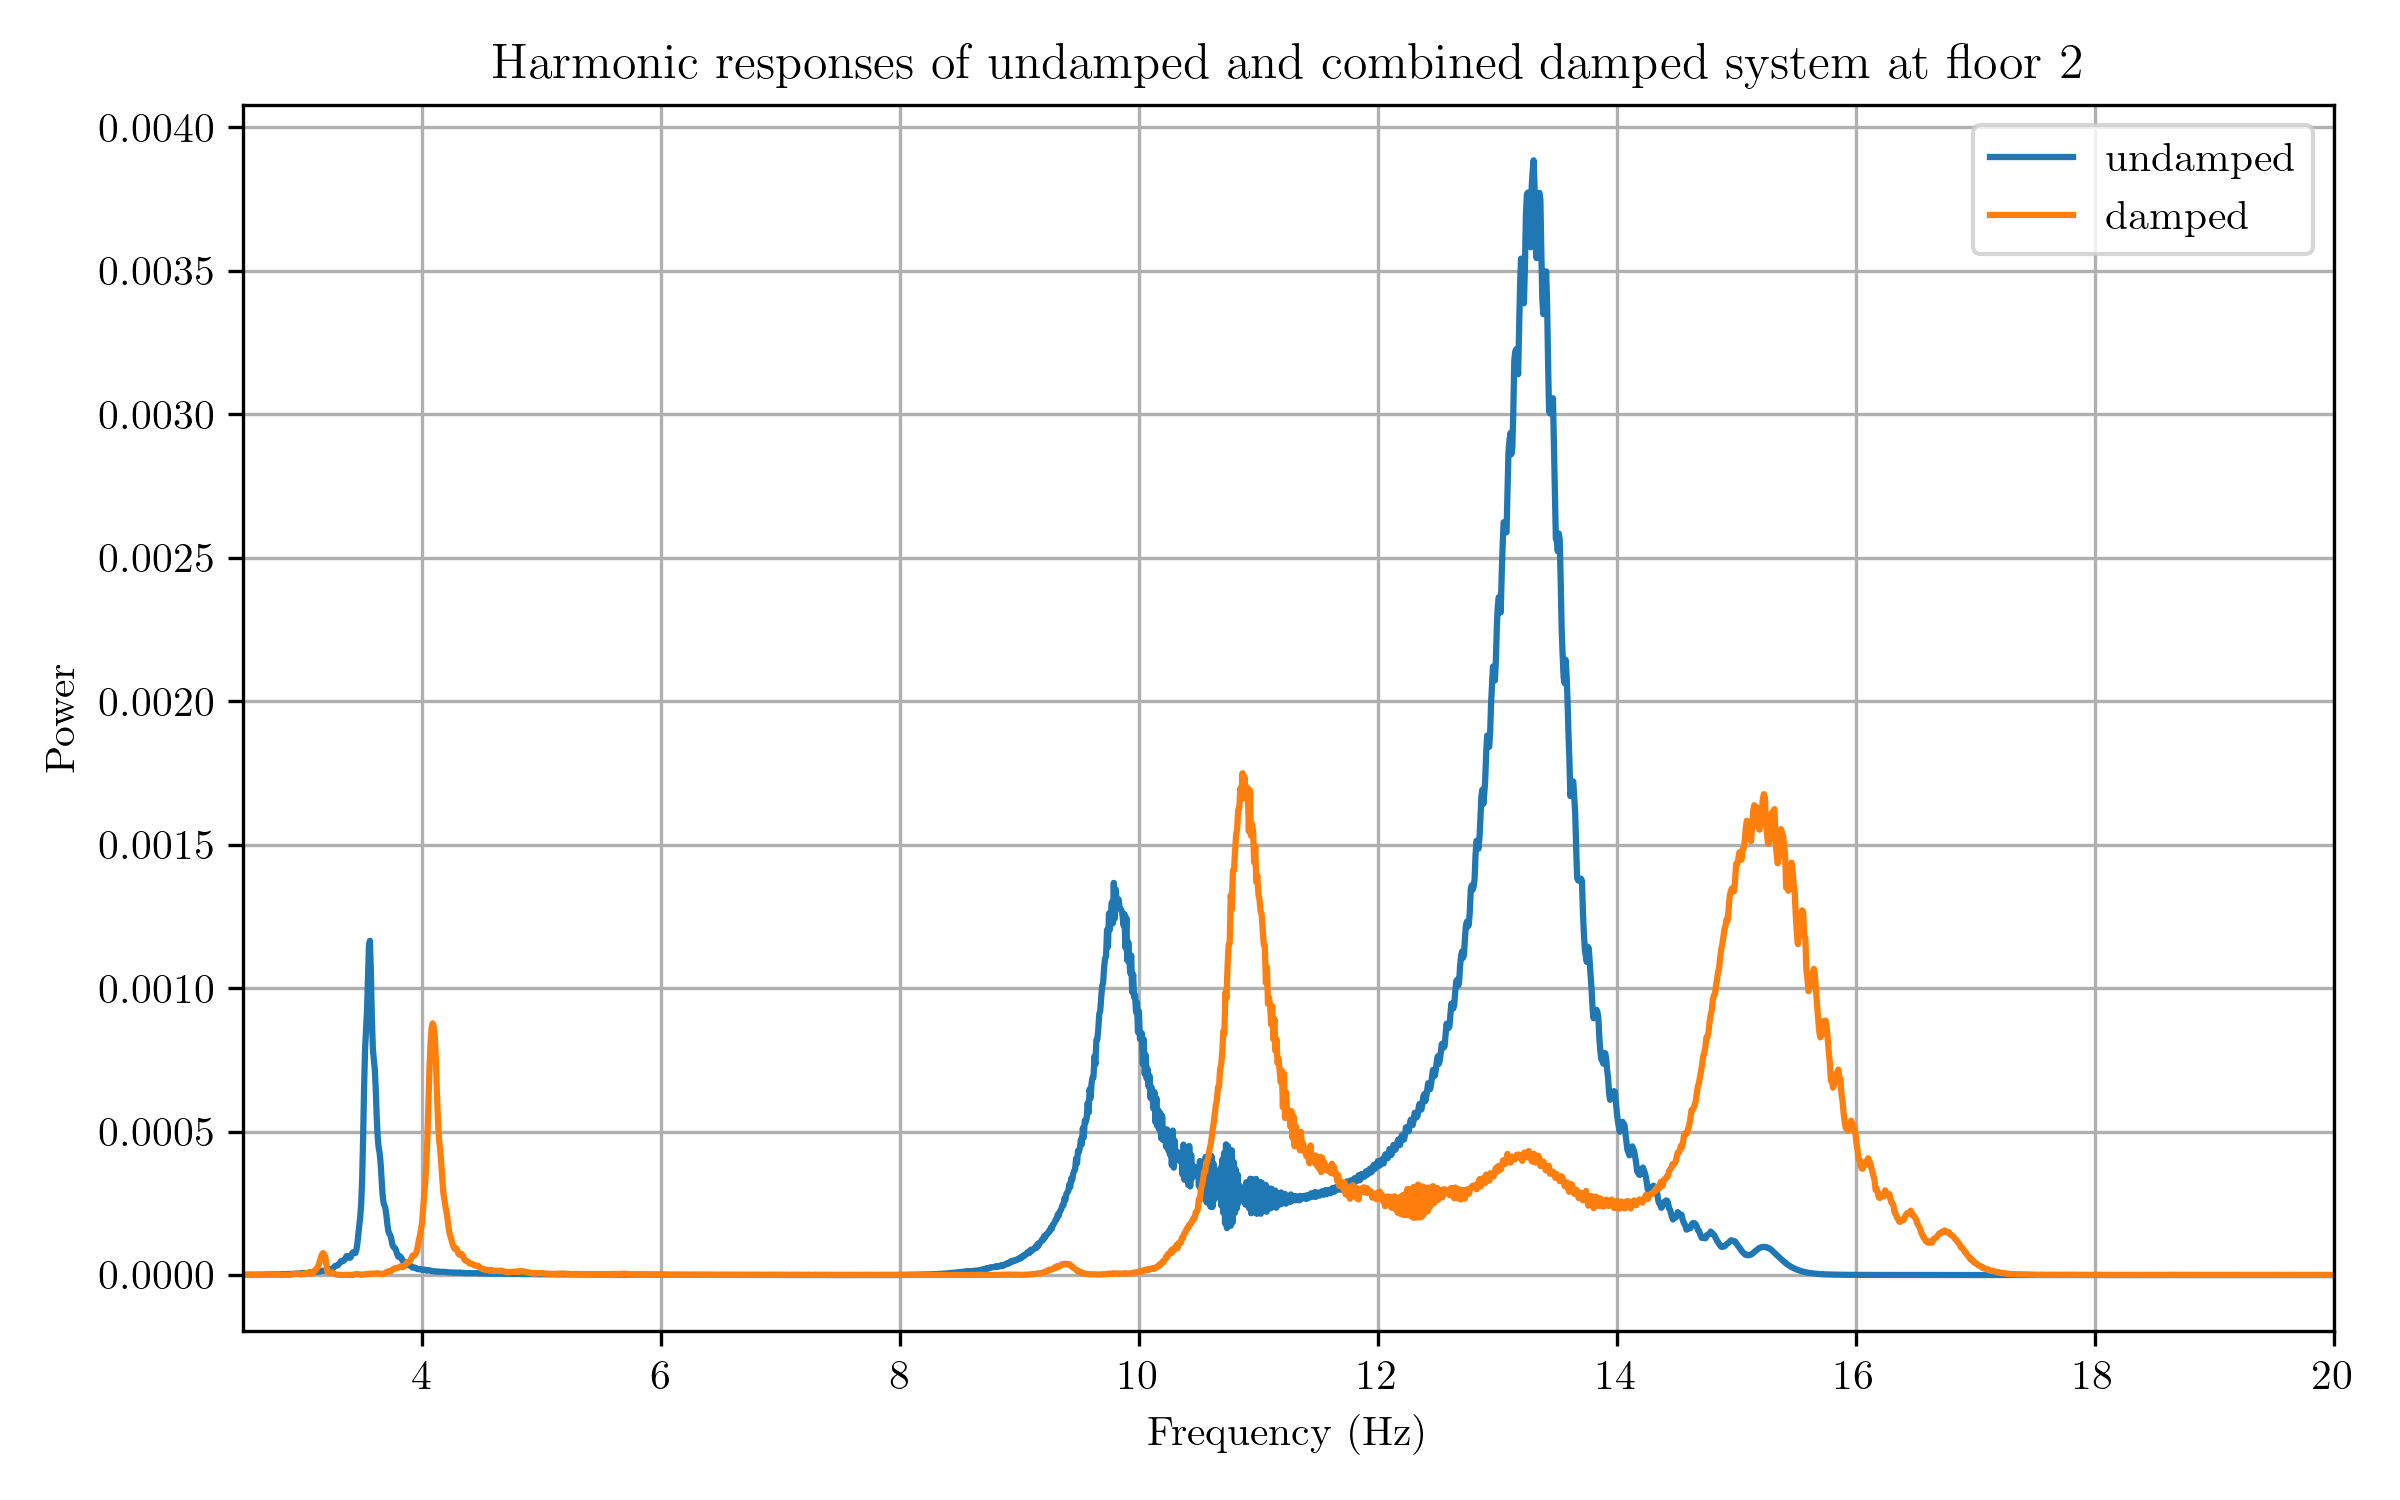
\includegraphics[width=0.8\textwidth]{combined_full_sweep.png}
    \caption{\label{fig:combined_full_sweep} Harmonic response of structure before and after the addition of 3 tuned dampers}
\end{figure}

\newpage
\section{Discussion}
%interpret results and comment on anomalies

Figure \ref{fig:modes} shows the resonant response of each mode before and after the addition of a tuned mass damper.
In all cases the response at the resonant frequency is reduced by the addition of the tuned mass damper. It can also be seen that the
response slightly above and below the resonant frequency increases. This is the expected behaviour from adding a tuned mass damper.
However, in modes 1 and 2 the new resonant response is greater than the original response.

This is likely due to a variety of reasons:
\begin{itemize}
    \item The tuned mass dampers were not accurately tuned to the resonant frequency of the structure. Our tuning method was not optimal as the length of the cantilever was only tuned to the nearest 5mm.
            This was done to reduce the time taken to tune the dampers as the tuning method was already very time consuming.
    \item The damping of the masses is very small as the air friction is negligible. This means that the two residual resonant responses are much higher than they would be if the absorbers had damping.
\end{itemize}

Figure \ref{fig:combined_full_sweep} shows the resonant response of the structure before and after the addition of the 3 individually tuned mass dampers.
Second order effects are seen in the response of the damped structure.

\section{Improvements}

The tuning method used to tune the tuned mass dampers was not optimal and could be improved.
This could be done by tuning the length of the cantilever to a higher precision using callipers.
Using a more accurate model of the tuned mass damper

\section{Conclusion}

From the experimental data gathered it can be concluded that tuned mass dampers can be used to reduce the amplitude of resonant responses of a structure.
However, tuning such dampers to the resonant frequency of the structure is not trivial and requires a lot of experimentation.

\end{document}
